\documentclass[11pt]{article}
\usepackage[utf8]{inputenc}
\usepackage[T1]{fontenc}
\usepackage{amsmath}
\usepackage{amssymb}
\usepackage{multicol}
\usepackage{geometry}
\usepackage{tikz}
\usepackage{enumitem}
\usepackage{xcolor}
\usepackage{titlesec}
\usepackage{parskip}
\usepackage{tcolorbox}
\tcbset{colback=white}

% Configurações de layout
\geometry{a4paper, left=1cm, right=1cm, top=0.5cm, bottom=1.2cm}
\setlength{\columnseprule}{0.4pt}

% Cores para títulos
\titleformat{\section}{\normalfont\Large\bfseries\color{blue}}{\thesection}{1em}{}
\titleformat{\subsection}{\normalfont\large\bfseries\color{red}}{\thesubsection}{1em}{}

\title{\textcolor{red}{Terceiro Trimestre: Matemática
    \\Medidas de Tendência Central - Revisão}}
\author{Professor: Jefferson}
\date{}

\begin{document}

\maketitle
\vspace{-1cm}

%\begin{center}
%\large{Nome: \underline{\hspace{8cm}} \quad Turma: \underline{\hspace{3cm}}}
%\end{center}

\begin{multicols}{2}

\section*{Fórmulas Importantes}

\subsection*{Média Aritmética}

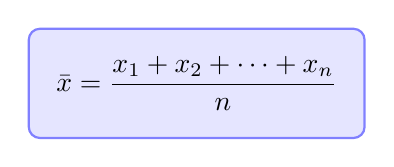
\begin{tikzpicture}
\node[rectangle, fill=blue!10, rounded corners, inner sep=10pt, draw=blue!50, thick] (box) {
$\displaystyle \bar{x} = \frac{x_1 + x_2 + \cdots + x_n}{n}$
};
\end{tikzpicture}

\textbf{Onde:}
\begin{itemize}
\item $\bar{x}$ = média aritmética
\item $x_1, x_2, \ldots, x_n$ = valores dos dados
\item $n$ = número total de dados
\end{itemize}

\subsection*{Mediana}

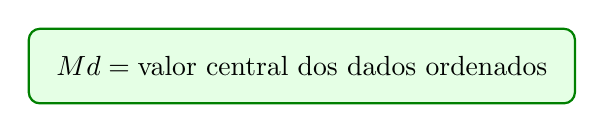
\begin{tikzpicture}
\node[rectangle, fill=green!10, rounded corners, inner sep=10pt, draw=green!50!black, thick] (box) {
$\displaystyle Md = \text{valor central dos dados ordenados}$
};
\end{tikzpicture}

\textbf{Procedimento:}
\begin{enumerate}
\item Ordene os dados em ordem crescente
\item Se $n$ é ímpar: $Md = \text{valor do meio}$
\item Se $n$ é par: $Md = \frac{\text{dois valores centrais}}{2}$
\end{enumerate}

\subsection*{Moda}

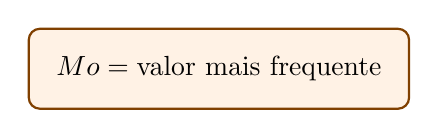
\begin{tikzpicture}
\node[rectangle, fill=orange!10, rounded corners, inner sep=10pt, draw=orange!50!black, thick] (box) {
$\displaystyle Mo = \text{valor mais frequente}$
};
\end{tikzpicture}

\textbf{Tipos:}
\begin{itemize}
\item Amodal: nenhuma moda
\item Unimodal: uma moda
\item Bimodal: duas modas
\item Multimodal: três ou mais modas
\end{itemize}

\section*{Exercícios Básicos}

\begin{enumerate}[leftmargin=*]

\item Calcule a média aritmética dos seguintes conjuntos:
\begin{enumerate}[label=\alph*)]
\item $4, 7, 9, 12, 18$
\item $8, 8, 10, 12, 14, 18$
\item $5, 10, 15, 20, 25$
\end{enumerate}

\item Determine a mediana dos conjuntos:
\begin{enumerate}[label=\alph*)]
\item $6, 2, 8, 4, 10$ (ordene primeiro)
\item $15, 20, 25, 30, 35, 40$
\item $3, 7, 1, 9, 5, 8, 2$
\end{enumerate}

\item Encontre a moda dos conjuntos:
\begin{enumerate}[label=\alph*)]
\item $4, 6, 4, 8, 4, 10, 6$
\item $12, 15, 18, 15, 20, 12, 25$
\item $7, 9, 11, 13, 15$ (classifique)
\end{enumerate}

\item Dado o conjunto: $5, 8, 8, 12, 15, 8, 20$, calcule:
\begin{enumerate}[label=\alph*)]
\item Média
\item Mediana
\item Moda
\end{enumerate}

\item Resolva os problemas:
\begin{enumerate}[label=\alph*)]
\item As alturas de 4 amigos são: 165, 170, 175, 180 cm. Qual a média de altura?
\item Se Maria tira notas 5, 6, 7, qual deve ser sua 4ª nota para ter média 6,5?
\end{enumerate}

\item Analise e compare os conjuntos:

\textbf{Conjunto A:} $12, 14, 16, 18, 20$

\textbf{Conjunto B:} $12, 12, 12, 20, 24$

\begin{enumerate}[label=\alph*)]
\item Calcule média, mediana e moda de cada
\item Qual conjunto é mais homogêneo?
\end{enumerate}

\item Problemas contextualizados:
\begin{enumerate}[label=\alph*)]
\item Um jogador fez nos últimos 5 jogos: 8, 12, 6, 10, 14 pontos. Qual sua média?
\item As idades de uma família: 12, 15, 18, 42, 45 anos. Encontre as 3 medidas.
\end{enumerate}

\item Identifique em cada caso qual medida é mais adequada:
\begin{enumerate}[label=\alph*)]
\item Salários de uma empresa pequena
\item Notas de uma prova difícil
\item Cor de camiseta mais popular na escola
\end{enumerate}

\item Calcule as três medidas para:
\begin{enumerate}[label=\alph*)]
\item $10, 15, 20, 25, 30, 35, 40$
\item $3, 4, 4, 5, 6, 6, 6, 7, 8$
\item $50, 60, 70, 80, 90$
\end{enumerate}

\end{enumerate}

\section*{Resoluções }

% Para manter a largura apropriada dentro das colunas, usamos 0.9\columnwidth
% Questão 1 a)
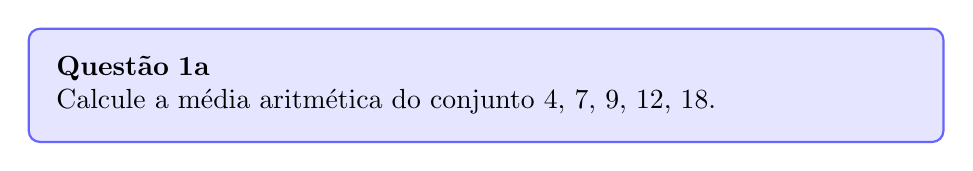
\begin{tikzpicture}
\node[rectangle, fill=blue!10, rounded corners, inner sep=10pt, draw=blue!60, thick, text width=0.9\columnwidth] (Q1a) {
\textbf{Questão 1a}\\
Calcule a média aritmética do conjunto $4,\,7,\,9,\,12,\,18$.
};
\end{tikzpicture}

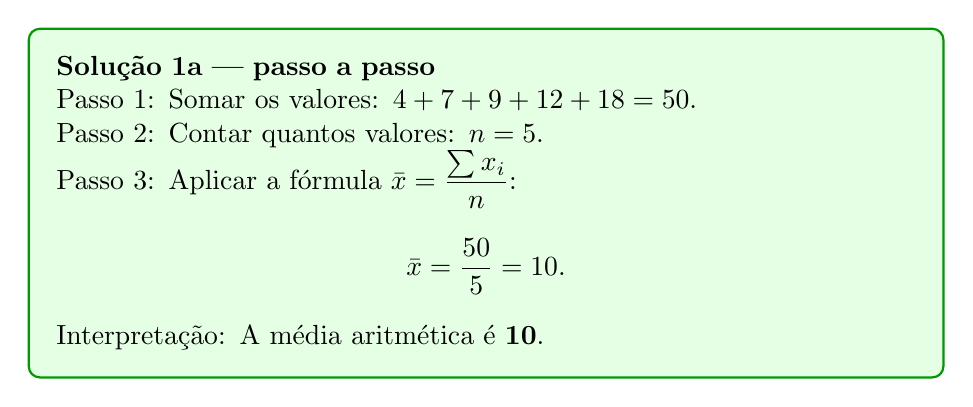
\begin{tikzpicture}
\node[rectangle, fill=green!10, rounded corners, inner sep=10pt, draw=green!60!black, thick, text width=0.9\columnwidth] (S1a) {
\textbf{Solução 1a — passo a passo}\\
Passo 1: Somar os valores: $4+7+9+12+18 = 50$.\\
Passo 2: Contar quantos valores: $n=5$.\\
Passo 3: Aplicar a fórmula $\bar{x} = \dfrac{\sum x_i}{n}$:
\[
\bar{x} = \frac{50}{5} = 10.
\]
Interpretação: A média aritmética é \textbf{10}.
};
\end{tikzpicture}

% Questão 1 b)
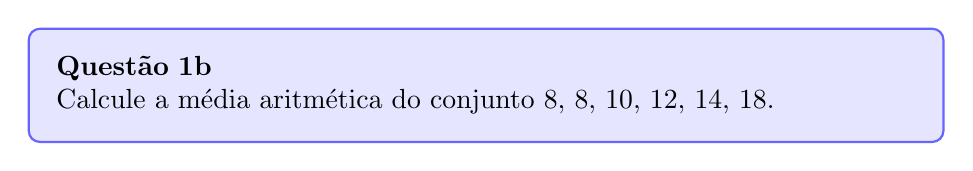
\begin{tikzpicture}
\node[rectangle, fill=blue!10, rounded corners, inner sep=10pt, draw=blue!60, thick, text width=0.9\columnwidth] (Q1b) {
\textbf{Questão 1b}\\
Calcule a média aritmética do conjunto $8,\,8,\,10,\,12,\,14,\,18$.
};
\end{tikzpicture}

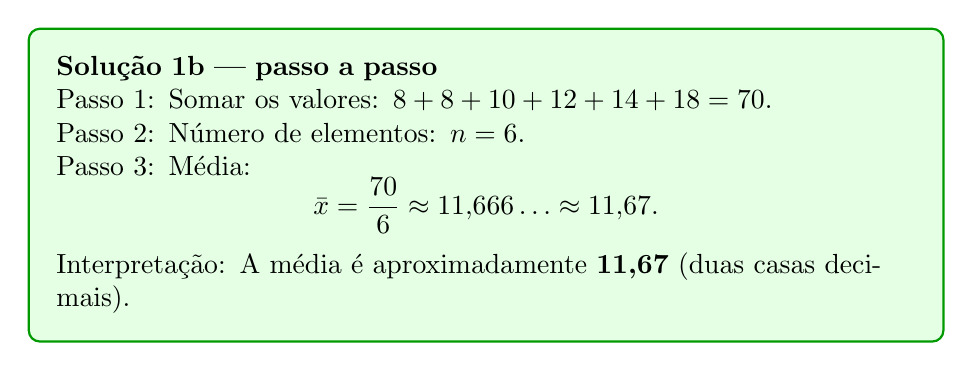
\begin{tikzpicture}
\node[rectangle, fill=green!10, rounded corners, inner sep=10pt, draw=green!60!black, thick, text width=0.9\columnwidth] (S1b) {
\textbf{Solução 1b — passo a passo}\\
Passo 1: Somar os valores: $8+8+10+12+14+18 = 70$.\\
Passo 2: Número de elementos: $n=6$.\\
Passo 3: Média:
\[
\bar{x} = \frac{70}{6} \approx 11{,}666\ldots \approx 11{,}67.
\]
Interpretação: A média é aproximadamente \textbf{11,67} (duas casas decimais).
};
\end{tikzpicture}

% Questão 1 c)
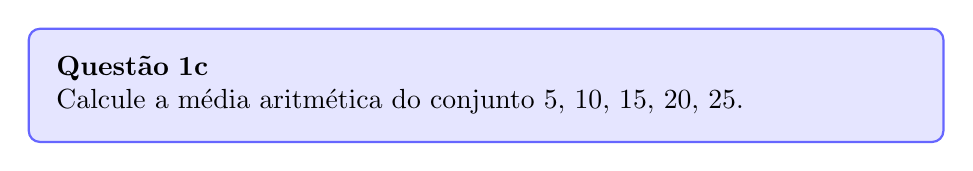
\begin{tikzpicture}
\node[rectangle, fill=blue!10, rounded corners, inner sep=10pt, draw=blue!60, thick, text width=0.9\columnwidth] (Q1c) {
\textbf{Questão 1c}\\
Calcule a média aritmética do conjunto $5,\,10,\,15,\,20,\,25$.
};
\end{tikzpicture}

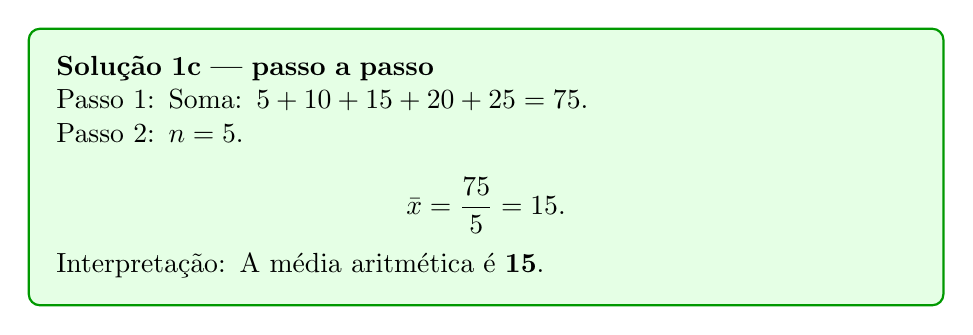
\begin{tikzpicture}
\node[rectangle, fill=green!10, rounded corners, inner sep=10pt, draw=green!60!black, thick, text width=0.9\columnwidth] (S1c) {
\textbf{Solução 1c — passo a passo}\\
Passo 1: Soma: $5+10+15+20+25 = 75$.\\
Passo 2: $n=5$.\\
\[
\bar{x} = \frac{75}{5} = 15.
\]
Interpretação: A média aritmética é \textbf{15}.
};
\end{tikzpicture}

% Questão 2 a)
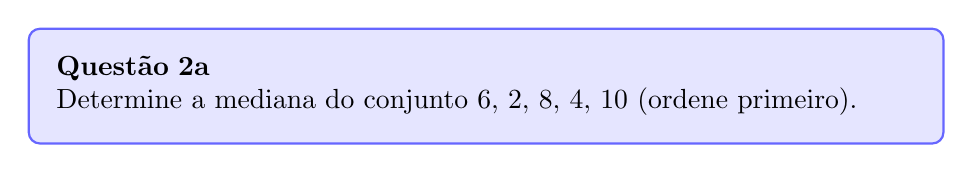
\begin{tikzpicture}
\node[rectangle, fill=blue!10, rounded corners, inner sep=10pt, draw=blue!60, thick, text width=0.9\columnwidth] (Q2a) {
\textbf{Questão 2a}\\
Determine a mediana do conjunto $6,\,2,\,8,\,4,\,10$ (ordene primeiro).
};
\end{tikzpicture}

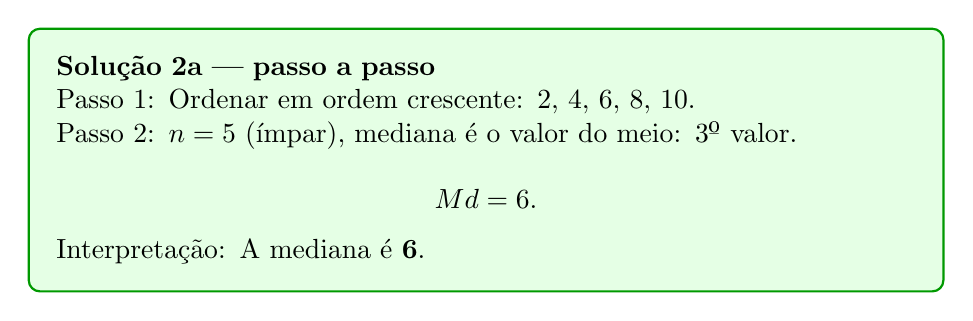
\begin{tikzpicture}
\node[rectangle, fill=green!10, rounded corners, inner sep=10pt, draw=green!60!black, thick, text width=0.9\columnwidth] (S2a) {
\textbf{Solução 2a — passo a passo}\\
Passo 1: Ordenar em ordem crescente: $2,\,4,\,6,\,8,\,10$.\\
Passo 2: $n=5$ (ímpar), mediana é o valor do meio: 3º valor.\\
\[
Md = 6.
\]
Interpretação: A mediana é \textbf{6}.
};
\end{tikzpicture}

% Questão 2 b)
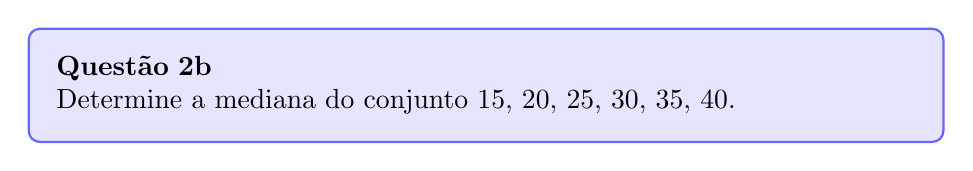
\begin{tikzpicture}
\node[rectangle, fill=blue!10, rounded corners, inner sep=10pt, draw=blue!60, thick, text width=0.9\columnwidth] (Q2b) {
\textbf{Questão 2b}\\
Determine a mediana do conjunto $15,\,20,\,25,\,30,\,35,\,40$.
};
\end{tikzpicture}

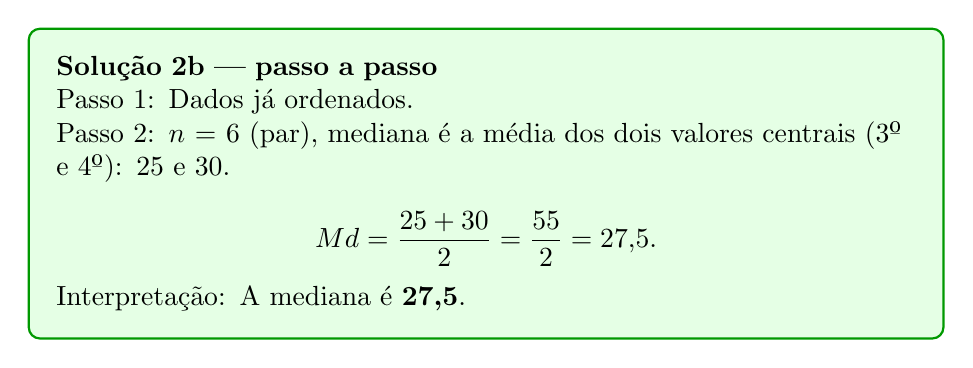
\begin{tikzpicture}
\node[rectangle, fill=green!10, rounded corners, inner sep=10pt, draw=green!60!black, thick, text width=0.9\columnwidth] (S2b) {
\textbf{Solução 2b — passo a passo}\\
Passo 1: Dados já ordenados.\\
Passo 2: $n=6$ (par), mediana é a média dos dois valores centrais (3º e 4º): 25 e 30.\\
\[
Md = \frac{25+30}{2} = \frac{55}{2} = 27{,}5.
\]
Interpretação: A mediana é \textbf{27,5}.
};
\end{tikzpicture}

% Questão 2 c)
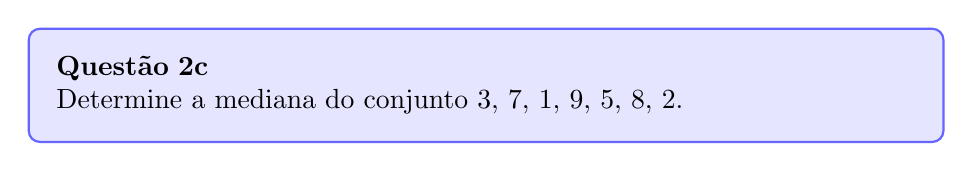
\begin{tikzpicture}
\node[rectangle, fill=blue!10, rounded corners, inner sep=10pt, draw=blue!60, thick, text width=0.9\columnwidth] (Q2c) {
\textbf{Questão 2c}\\
Determine a mediana do conjunto $3,\,7,\,1,\,9,\,5,\,8,\,2$.
};
\end{tikzpicture}

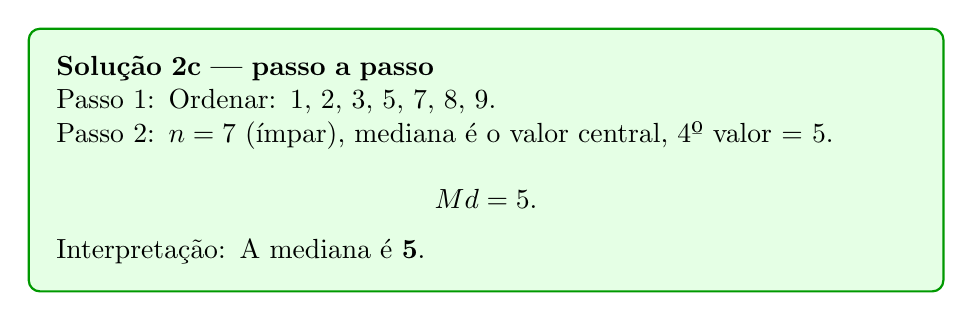
\begin{tikzpicture}
\node[rectangle, fill=green!10, rounded corners, inner sep=10pt, draw=green!60!black, thick, text width=0.9\columnwidth] (S2c) {
\textbf{Solução 2c — passo a passo}\\
Passo 1: Ordenar: $1,\,2,\,3,\,5,\,7,\,8,\,9$.\\
Passo 2: $n=7$ (ímpar), mediana é o valor central, 4º valor = 5.\\
\[
Md = 5.
\]
Interpretação: A mediana é \textbf{5}.
};
\end{tikzpicture}

% Questão 3 a)
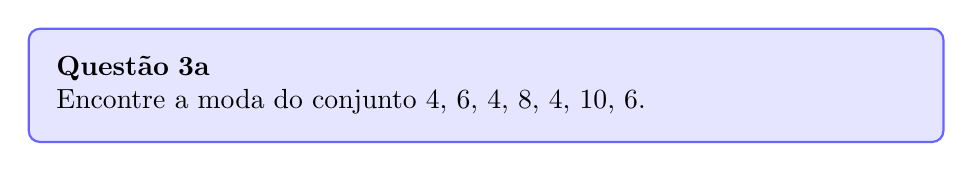
\begin{tikzpicture}
\node[rectangle, fill=blue!10, rounded corners, inner sep=10pt, draw=blue!60, thick, text width=0.9\columnwidth] (Q3a) {
\textbf{Questão 3a}\\
Encontre a moda do conjunto $4,\,6,\,4,\,8,\,4,\,10,\,6$.
};
\end{tikzpicture}

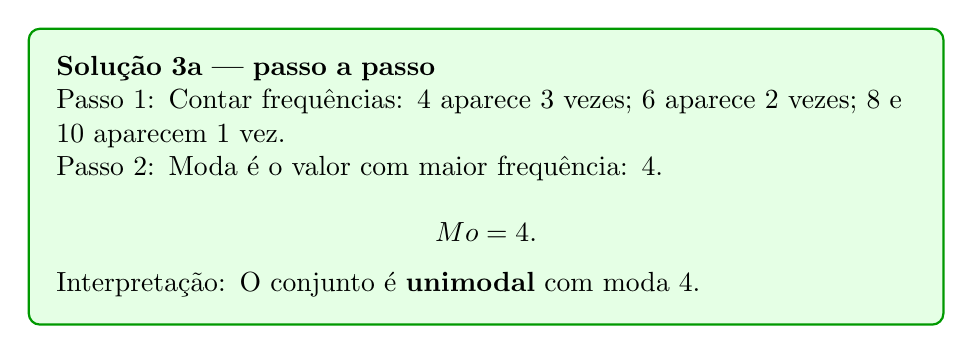
\begin{tikzpicture}
\node[rectangle, fill=green!10, rounded corners, inner sep=10pt, draw=green!60!black, thick, text width=0.9\columnwidth] (S3a) {
\textbf{Solução 3a — passo a passo}\\
Passo 1: Contar frequências: 4 aparece 3 vezes; 6 aparece 2 vezes; 8 e 10 aparecem 1 vez.\\
Passo 2: Moda é o valor com maior frequência: 4.\\
\[
Mo = 4.
\]
Interpretação: O conjunto é \textbf{unimodal} com moda 4.
};
\end{tikzpicture}

% Questão 3 b)
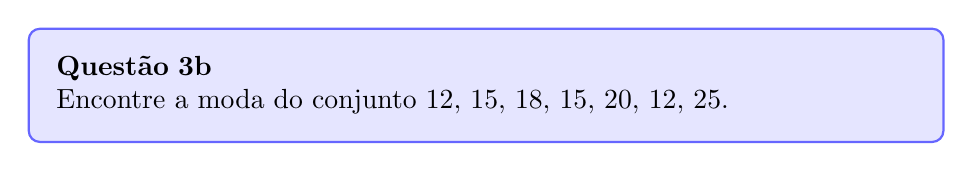
\begin{tikzpicture}
\node[rectangle, fill=blue!10, rounded corners, inner sep=10pt, draw=blue!60, thick, text width=0.9\columnwidth] (Q3b) {
\textbf{Questão 3b}\\
Encontre a moda do conjunto $12,\,15,\,18,\,15,\,20,\,12,\,25$.
};
\end{tikzpicture}

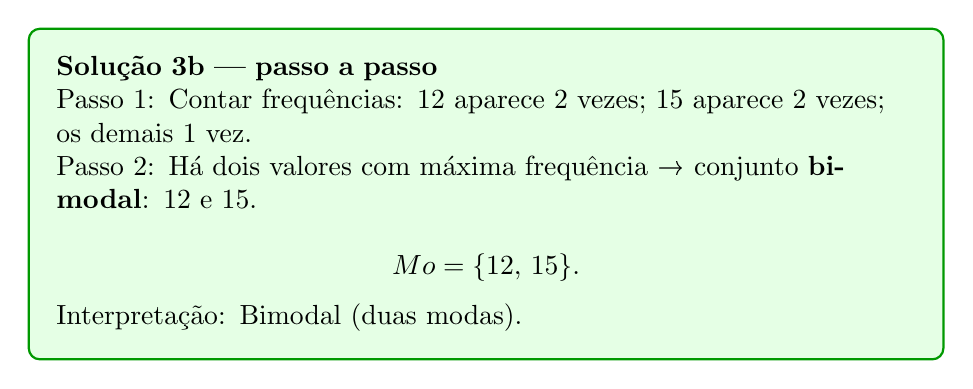
\begin{tikzpicture}
\node[rectangle, fill=green!10, rounded corners, inner sep=10pt, draw=green!60!black, thick, text width=0.9\columnwidth] (S3b) {
\textbf{Solução 3b — passo a passo}\\
Passo 1: Contar frequências: 12 aparece 2 vezes; 15 aparece 2 vezes; os demais 1 vez.\\
Passo 2: Há dois valores com máxima frequência → conjunto \textbf{bimodal}: 12 e 15.\\
\[
Mo = \{12,\,15\}.
\]
Interpretação: Bimodal (duas modas).
};
\end{tikzpicture}

% Questão 3 c)
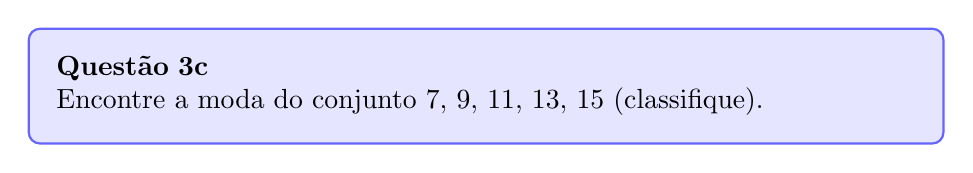
\begin{tikzpicture}
\node[rectangle, fill=blue!10, rounded corners, inner sep=10pt, draw=blue!60, thick, text width=0.9\columnwidth] (Q3c) {
\textbf{Questão 3c}\\
Encontre a moda do conjunto $7,\,9,\,11,\,13,\,15$ (classifique).
};
\end{tikzpicture}

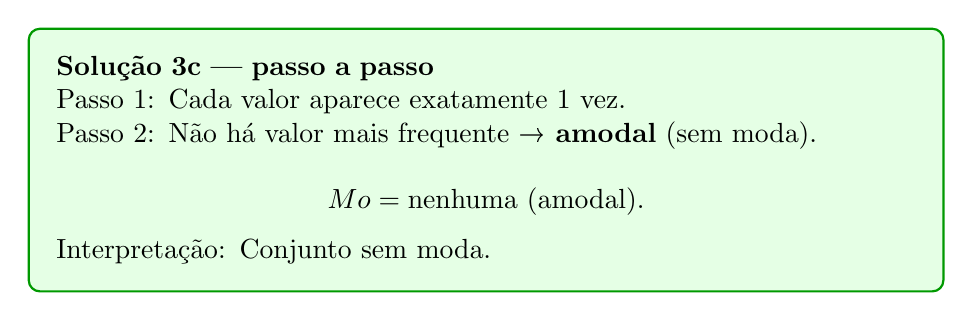
\begin{tikzpicture}
\node[rectangle, fill=green!10, rounded corners, inner sep=10pt, draw=green!60!black, thick, text width=0.9\columnwidth] (S3c) {
\textbf{Solução 3c — passo a passo}\\
Passo 1: Cada valor aparece exatamente 1 vez.\\
Passo 2: Não há valor mais frequente → \textbf{amodal} (sem moda).\\
\[
Mo = \text{nenhuma (amodal)}.
\]
Interpretação: Conjunto sem moda.
};
\end{tikzpicture}

% Questão 4 a)
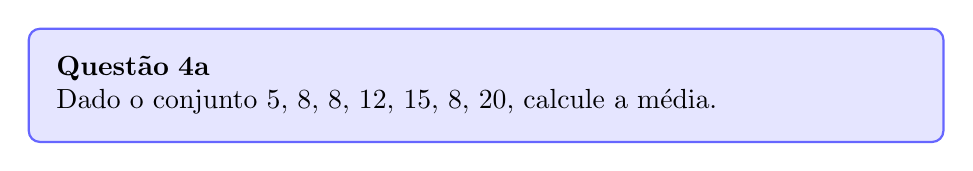
\begin{tikzpicture}
\node[rectangle, fill=blue!10, rounded corners, inner sep=10pt, draw=blue!60, thick, text width=0.9\columnwidth] (Q4a) {
\textbf{Questão 4a}\\
Dado o conjunto $5,\,8,\,8,\,12,\,15,\,8,\,20$, calcule a média.
};
\end{tikzpicture}

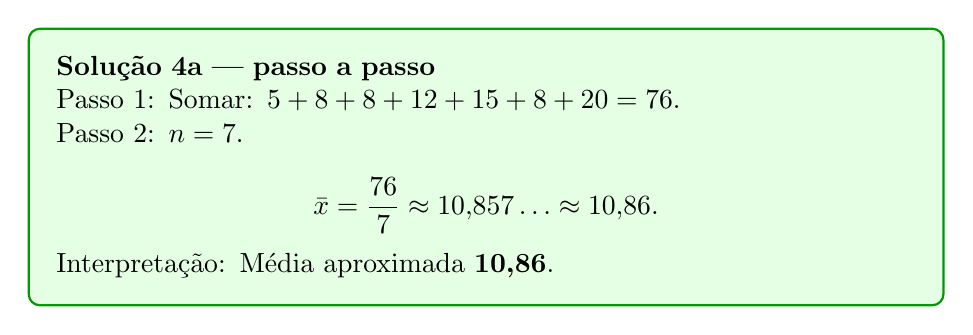
\begin{tikzpicture}
\node[rectangle, fill=green!10, rounded corners, inner sep=10pt, draw=green!60!black, thick, text width=0.9\columnwidth] (S4a) {
\textbf{Solução 4a — passo a passo}\\
Passo 1: Somar: $5+8+8+12+15+8+20 = 76$.\\
Passo 2: $n=7$.\\
\[
\bar{x} = \frac{76}{7} \approx 10{,}857\ldots \approx 10{,}86.
\]
Interpretação: Média aproximada \textbf{10,86}.
};
\end{tikzpicture}

% Questão 4 b)
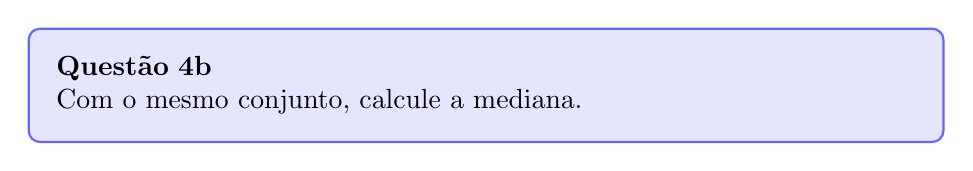
\begin{tikzpicture}
\node[rectangle, fill=blue!10, rounded corners, inner sep=10pt, draw=blue!60, thick, text width=0.9\columnwidth] (Q4b) {
\textbf{Questão 4b}\\
Com o mesmo conjunto, calcule a mediana.
};
\end{tikzpicture}

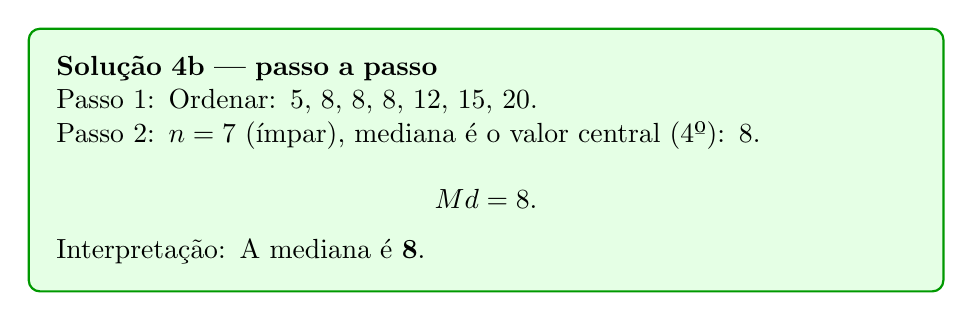
\begin{tikzpicture}
\node[rectangle, fill=green!10, rounded corners, inner sep=10pt, draw=green!60!black, thick, text width=0.9\columnwidth] (S4b) {
\textbf{Solução 4b — passo a passo}\\
Passo 1: Ordenar: $5,\,8,\,8,\,8,\,12,\,15,\,20$.\\
Passo 2: $n=7$ (ímpar), mediana é o valor central (4º): 8.\\
\[
Md = 8.
\]
Interpretação: A mediana é \textbf{8}.
};
\end{tikzpicture}

% Questão 4 c)
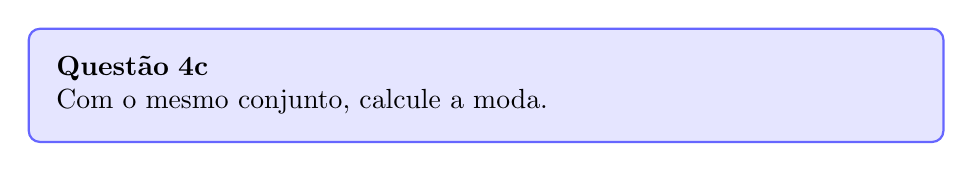
\begin{tikzpicture}
\node[rectangle, fill=blue!10, rounded corners, inner sep=10pt, draw=blue!60, thick, text width=0.9\columnwidth] (Q4c) {
\textbf{Questão 4c}\\
Com o mesmo conjunto, calcule a moda.
};
\end{tikzpicture}

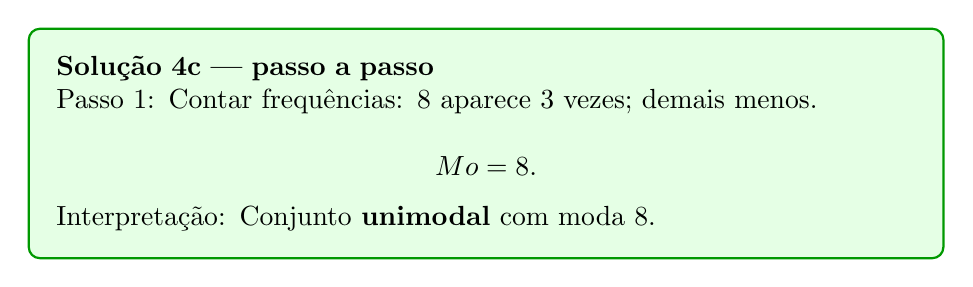
\begin{tikzpicture}
\node[rectangle, fill=green!10, rounded corners, inner sep=10pt, draw=green!60!black, thick, text width=0.9\columnwidth] (S4c) {
\textbf{Solução 4c — passo a passo}\\
Passo 1: Contar frequências: 8 aparece 3 vezes; demais menos.\\
\[
Mo = 8.
\]
Interpretação: Conjunto \textbf{unimodal} com moda 8.
};
\end{tikzpicture}

% Questão 5 a)
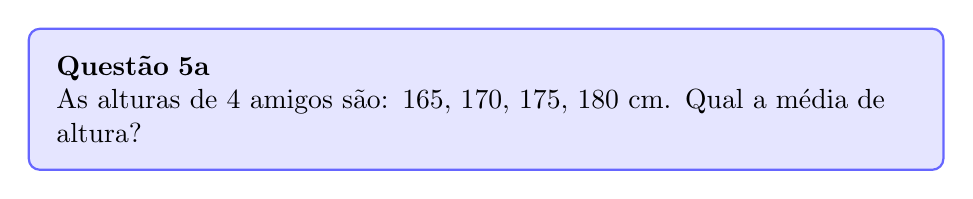
\begin{tikzpicture}
\node[rectangle, fill=blue!10, rounded corners, inner sep=10pt, draw=blue!60, thick, text width=0.9\columnwidth] (Q5a) {
\textbf{Questão 5a}\\
As alturas de 4 amigos são: $165,\,170,\,175,\,180$ cm. Qual a média de altura?
};
\end{tikzpicture}

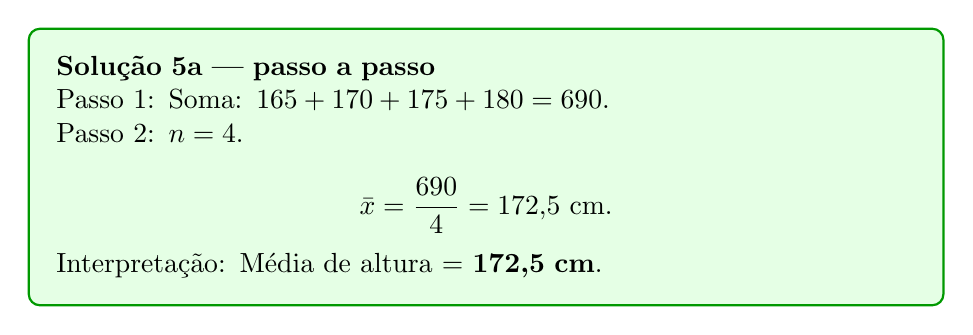
\begin{tikzpicture}
\node[rectangle, fill=green!10, rounded corners, inner sep=10pt, draw=green!60!black, thick, text width=0.9\columnwidth] (S5a) {
\textbf{Solução 5a — passo a passo}\\
Passo 1: Soma: $165+170+175+180 = 690$.\\
Passo 2: $n=4$.\\
\[
\bar{x} = \frac{690}{4} = 172{,}5 \text{ cm}.
\]
Interpretação: Média de altura = \textbf{172,5 cm}.
};
\end{tikzpicture}

% Questão 5 b)
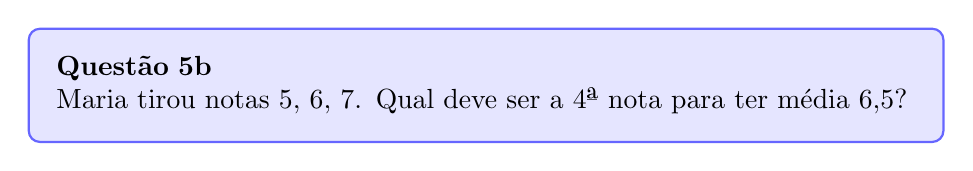
\begin{tikzpicture}
\node[rectangle, fill=blue!10, rounded corners, inner sep=10pt, draw=blue!60, thick, text width=0.9\columnwidth] (Q5b) {
\textbf{Questão 5b}\\
Maria tirou notas $5,\,6,\,7$. Qual deve ser a 4ª nota para ter média $6{,}5$?
};
\end{tikzpicture}

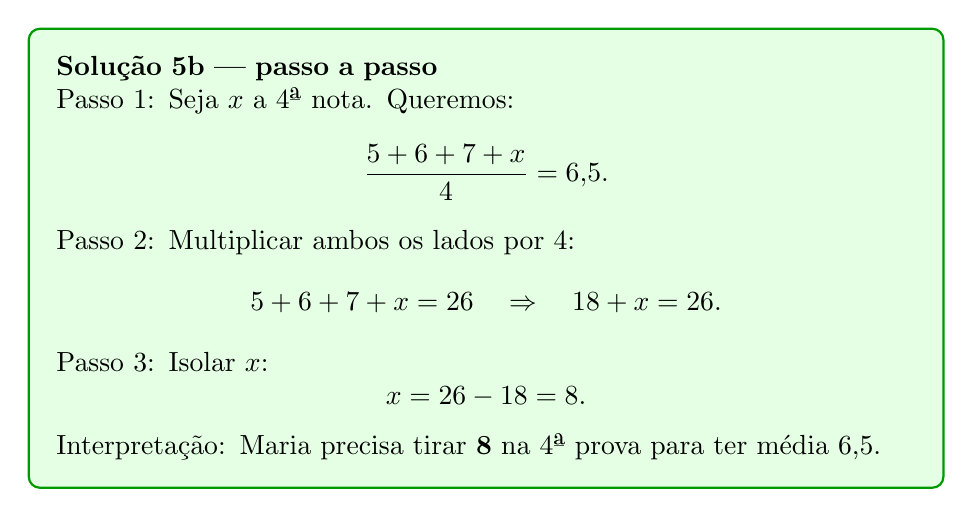
\begin{tikzpicture}
\node[rectangle, fill=green!10, rounded corners, inner sep=10pt, draw=green!60!black, thick, text width=0.9\columnwidth] (S5b) {
\textbf{Solução 5b — passo a passo}\\
Passo 1: Seja $x$ a 4ª nota. Queremos:
\[
\frac{5+6+7+x}{4} = 6{,}5.
\]
Passo 2: Multiplicar ambos os lados por 4:
\[
5+6+7+x = 26 \quad\Rightarrow\quad 18 + x = 26.
\]
Passo 3: Isolar $x$:
\[
x = 26 - 18 = 8.
\]
Interpretação: Maria precisa tirar \textbf{8} na 4ª prova para ter média 6,5.
};
\end{tikzpicture}

% Questão 6 a)
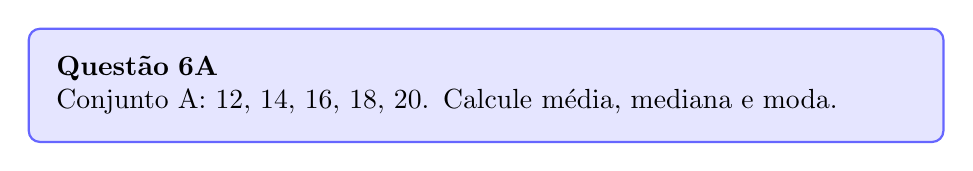
\begin{tikzpicture}
\node[rectangle, fill=blue!10, rounded corners, inner sep=10pt, draw=blue!60, thick, text width=0.9\columnwidth] (Q6a-Conjunto A) {
\textbf{Questão 6A}\\
Conjunto A: $12,\,14,\,16,\,18,\,20$. Calcule média, mediana e moda.
};
\end{tikzpicture}

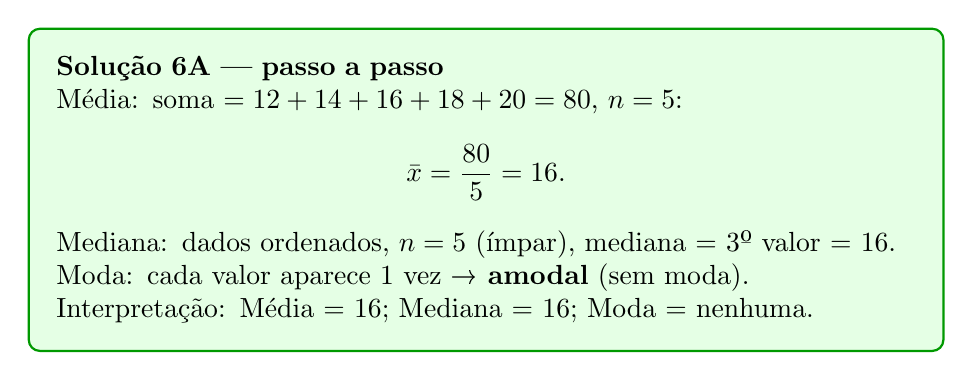
\begin{tikzpicture}
\node[rectangle, fill=green!10, rounded corners, inner sep=10pt, draw=green!60!black, thick, text width=0.9\columnwidth] (S6A) {
\textbf{Solução 6A — passo a passo}\\
Média: soma $=12+14+16+18+20=80$, $n=5$:
\[
\bar{x} = \frac{80}{5} = 16.
\]
Mediana: dados ordenados, $n=5$ (ímpar), mediana = 3º valor = 16.\\
Moda: cada valor aparece 1 vez → \textbf{amodal} (sem moda).\\
Interpretação: Média = 16; Mediana = 16; Moda = nenhuma.
};
\end{tikzpicture}

% Questão 6 b)
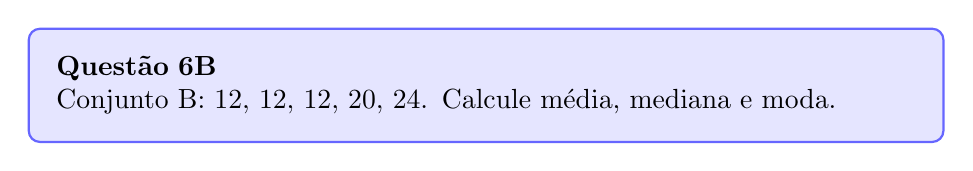
\begin{tikzpicture}
\node[rectangle, fill=blue!10, rounded corners, inner sep=10pt, draw=blue!60, thick, text width=0.9\columnwidth] (Q6B) {
\textbf{Questão 6B}\\
Conjunto B: $12,\,12,\,12,\,20,\,24$. Calcule média, mediana e moda.
};
\end{tikzpicture}

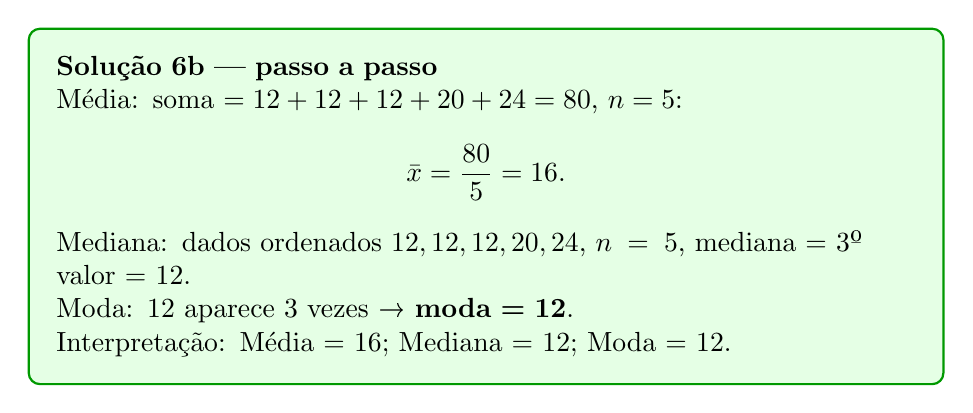
\begin{tikzpicture}
\node[rectangle, fill=green!10, rounded corners, inner sep=10pt, draw=green!60!black, thick, text width=0.9\columnwidth] (S6b) {
\textbf{Solução 6b — passo a passo}\\
Média: soma $=12+12+12+20+24=80$, $n=5$:
\[
\bar{x} = \frac{80}{5} = 16.
\]
Mediana: dados ordenados $12,12,12,20,24$, $n=5$, mediana = 3º valor = 12.\\
Moda: 12 aparece 3 vezes → \textbf{moda = 12}.\\
Interpretação: Média = 16; Mediana = 12; Moda = 12.
};
\end{tikzpicture}



% Questão 7 a)
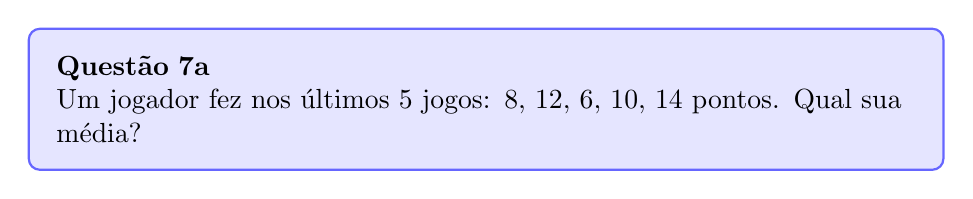
\begin{tikzpicture}
\node[rectangle, fill=blue!10, rounded corners, inner sep=10pt, draw=blue!60, thick, text width=0.9\columnwidth] (Q7a) {
\textbf{Questão 7a}\\
Um jogador fez nos últimos 5 jogos: $8,\,12,\,6,\,10,\,14$ pontos. Qual sua média?
};
\end{tikzpicture}

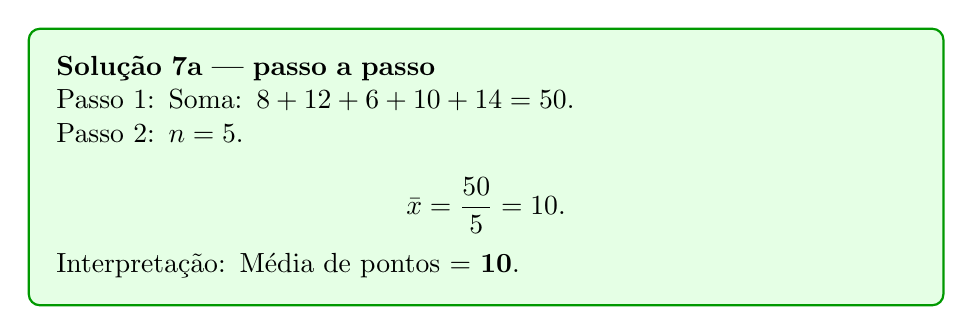
\begin{tikzpicture}
\node[rectangle, fill=green!10, rounded corners, inner sep=10pt, draw=green!60!black, thick, text width=0.9\columnwidth] (S7a) {
\textbf{Solução 7a — passo a passo}\\
Passo 1: Soma: $8+12+6+10+14 = 50$.\\
Passo 2: $n=5$.\\
\[
\bar{x} = \frac{50}{5} = 10.
\]
Interpretação: Média de pontos = \textbf{10}.
};
\end{tikzpicture}

% Questão 7 b)
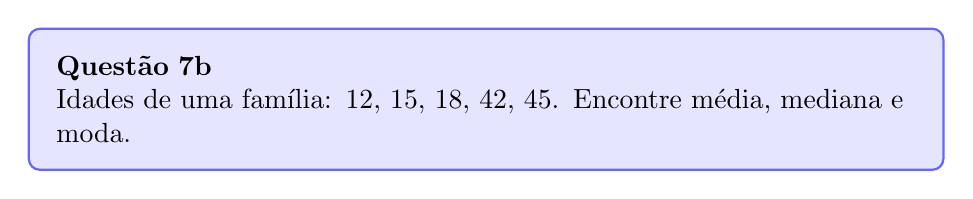
\begin{tikzpicture}
\node[rectangle, fill=blue!10, rounded corners, inner sep=10pt, draw=blue!60, thick, text width=0.9\columnwidth] (Q7b) {
\textbf{Questão 7b}\\
Idades de uma família: $12,\,15,\,18,\,42,\,45$. Encontre média, mediana e moda.
};
\end{tikzpicture}

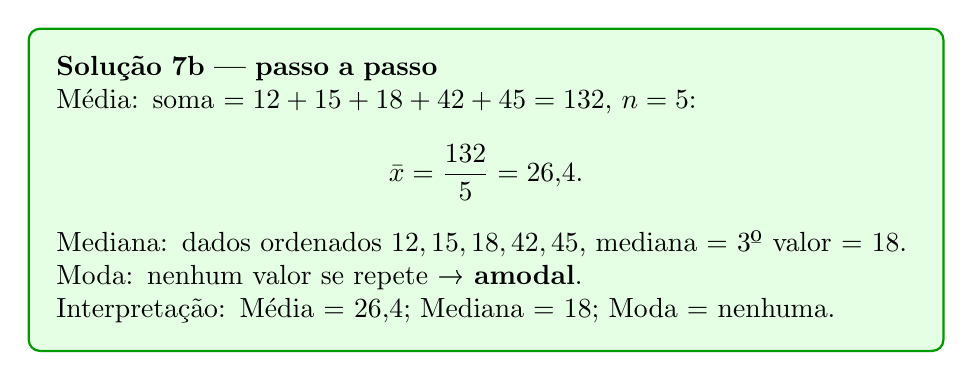
\begin{tikzpicture}
\node[rectangle, fill=green!10, rounded corners, inner sep=10pt, draw=green!60!black, thick, text width=0.9\columnwidth] (S7b) {
\textbf{Solução 7b — passo a passo}\\
Média: soma $=12+15+18+42+45 = 132$, $n=5$:
\[
\bar{x} = \frac{132}{5} = 26{,}4.
\]
Mediana: dados ordenados $12,15,18,42,45$, mediana = 3º valor = 18.\\
Moda: nenhum valor se repete → \textbf{amodal}.\\
Interpretação: Média = 26,4; Mediana = 18; Moda = nenhuma.
};
\end{tikzpicture}

% Questão 8 a)
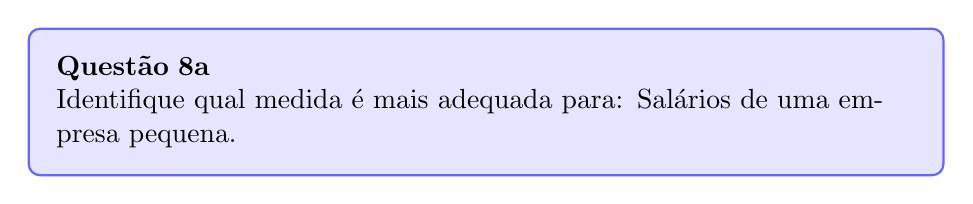
\begin{tikzpicture}
\node[rectangle, fill=blue!10, rounded corners, inner sep=10pt, draw=blue!60, thick, text width=0.9\columnwidth] (Q8a) {
\textbf{Questão 8a}\\
Identifique qual medida é mais adequada para: Salários de uma empresa pequena.
};
\end{tikzpicture}

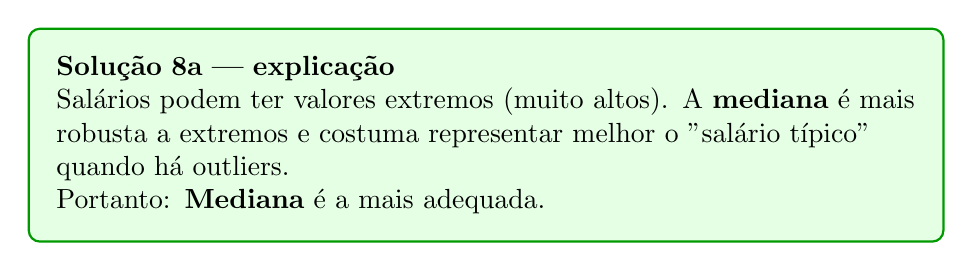
\begin{tikzpicture}
\node[rectangle, fill=green!10, rounded corners, inner sep=10pt, draw=green!60!black, thick, text width=0.9\columnwidth] (S8a) {
\textbf{Solução 8a — explicação}\\
Salários podem ter valores extremos (muito altos). A \textbf{mediana} é mais robusta a extremos e costuma representar melhor o "salário típico" quando há outliers.\\
Portanto: \textbf{Mediana} é a mais adequada.
};
\end{tikzpicture}

% Questão 8 b)
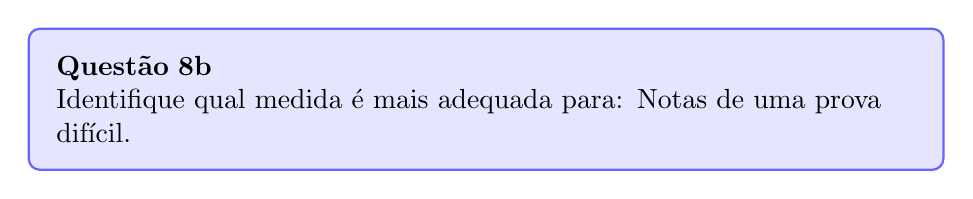
\begin{tikzpicture}
\node[rectangle, fill=blue!10, rounded corners, inner sep=10pt, draw=blue!60, thick, text width=0.9\columnwidth] (Q8b) {
\textbf{Questão 8b}\\
Identifique qual medida é mais adequada para: Notas de uma prova difícil.
};
\end{tikzpicture}

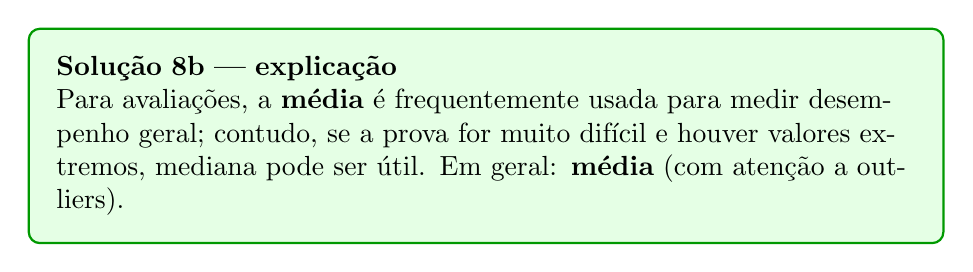
\begin{tikzpicture}
\node[rectangle, fill=green!10, rounded corners, inner sep=10pt, draw=green!60!black, thick, text width=0.9\columnwidth] (S8b) {
\textbf{Solução 8b — explicação}\\
Para avaliações, a \textbf{média} é frequentemente usada para medir desempenho geral; contudo, se a prova for muito difícil e houver valores extremos, mediana pode ser útil. Em geral: \textbf{média} (com atenção a outliers).
};
\end{tikzpicture}

% Questão 8 c)
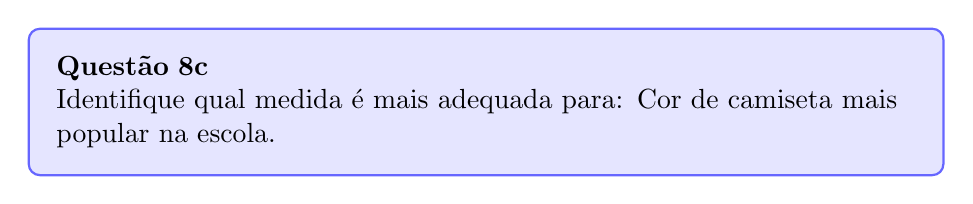
\begin{tikzpicture}
\node[rectangle, fill=blue!10, rounded corners, inner sep=10pt, draw=blue!60, thick, text width=0.9\columnwidth] (Q8c) {
\textbf{Questão 8c}\\
Identifique qual medida é mais adequada para: Cor de camiseta mais popular na escola.
};
\end{tikzpicture}

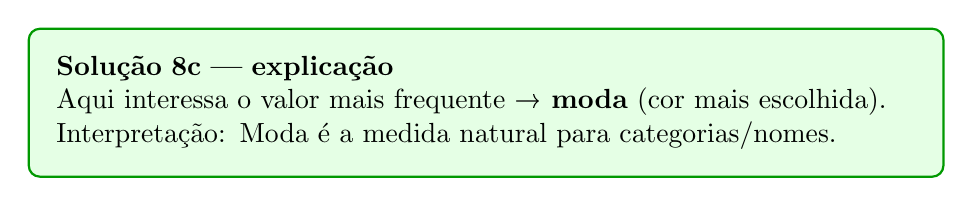
\begin{tikzpicture}
\node[rectangle, fill=green!10, rounded corners, inner sep=10pt, draw=green!60!black, thick, text width=0.9\columnwidth] (S8c) {
\textbf{Solução 8c — explicação}\\
Aqui interessa o valor mais frequente → \textbf{moda} (cor mais escolhida).\\
Interpretação: Moda é a medida natural para categorias/nomes.
};
\end{tikzpicture}

% Questão 9 a)
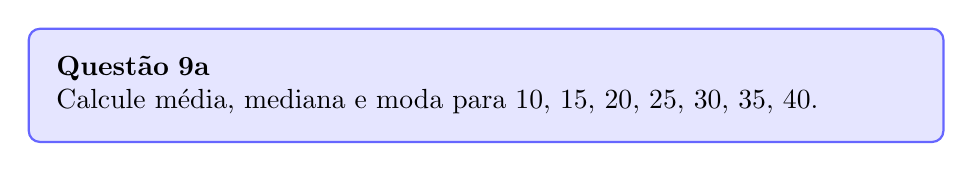
\begin{tikzpicture}
\node[rectangle, fill=blue!10, rounded corners, inner sep=10pt, draw=blue!60, thick, text width=0.9\columnwidth] (Q9a) {
\textbf{Questão 9a}\\
Calcule média, mediana e moda para $10,\,15,\,20,\,25,\,30,\,35,\,40$.
};
\end{tikzpicture}

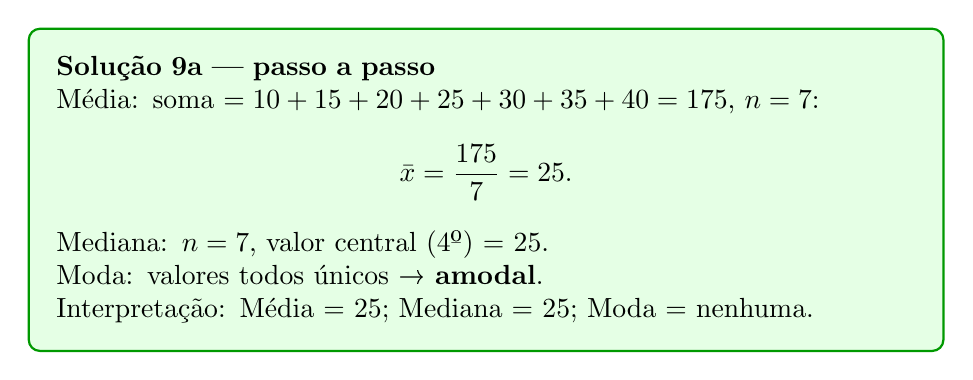
\begin{tikzpicture}
\node[rectangle, fill=green!10, rounded corners, inner sep=10pt, draw=green!60!black, thick, text width=0.9\columnwidth] (S9a) {
\textbf{Solução 9a — passo a passo}\\
Média: soma $=10+15+20+25+30+35+40=175$, $n=7$:
\[
\bar{x}=\frac{175}{7}=25.
\]
Mediana: $n=7$, valor central (4º) = 25.\\
Moda: valores todos únicos → \textbf{amodal}.\\
Interpretação: Média = 25; Mediana = 25; Moda = nenhuma.
};
\end{tikzpicture}

% Questão 9 b)
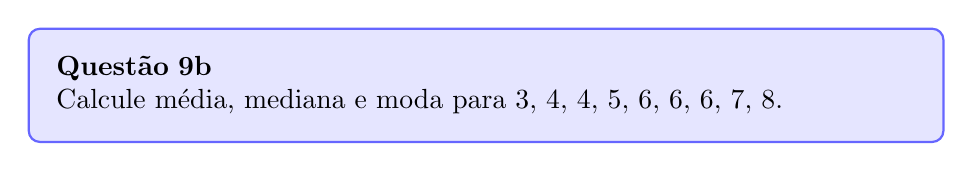
\begin{tikzpicture}
\node[rectangle, fill=blue!10, rounded corners, inner sep=10pt, draw=blue!60, thick, text width=0.9\columnwidth] (Q9b) {
\textbf{Questão 9b}\\
Calcule média, mediana e moda para $3,\,4,\,4,\,5,\,6,\,6,\,6,\,7,\,8$.
};
\end{tikzpicture}

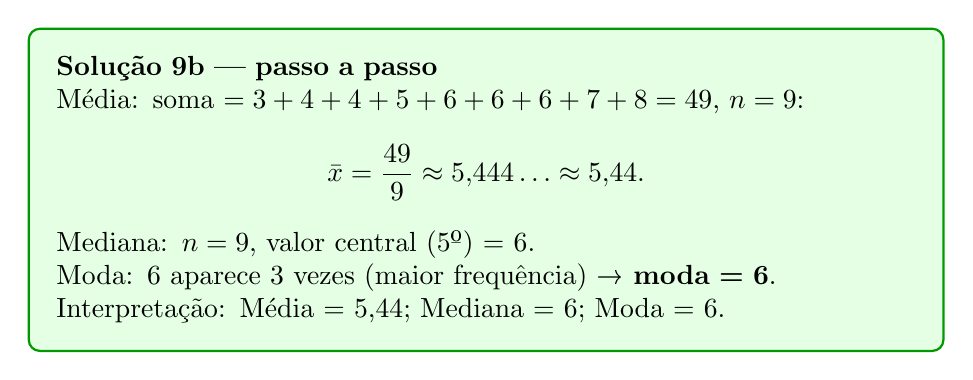
\begin{tikzpicture}
\node[rectangle, fill=green!10, rounded corners, inner sep=10pt, draw=green!60!black, thick, text width=0.9\columnwidth] (S9b) {
\textbf{Solução 9b — passo a passo}\\
Média: soma $=3+4+4+5+6+6+6+7+8 = 49$, $n=9$:
\[
\bar{x}=\frac{49}{9}\approx 5{,}444\ldots \approx 5{,}44.
\]
Mediana: $n=9$, valor central (5º) = 6.\\
Moda: 6 aparece 3 vezes (maior frequência) → \textbf{moda = 6}.\\
Interpretação: Média = 5,44; Mediana = 6; Moda = 6.
    };
\end{tikzpicture}

% Questão 9 c)
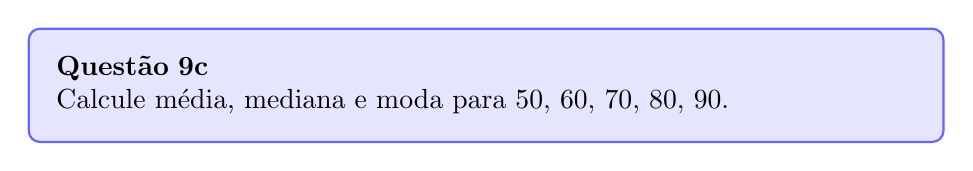
\begin{tikzpicture}
\node[rectangle, fill=blue!10, rounded corners, inner sep=10pt, draw=blue!60, thick, text width=0.9\columnwidth] (Q9c) {
\textbf{Questão 9c}\\
Calcule média, mediana e moda para $50,\,60,\,70,\,80,\,90$.
};
\end{tikzpicture}

\begin{tikzpicture}
\node[rectangle, fill=green!10, rounded corners, inner sep=10pt, draw=green!60!black, thick, text width=0.9\columnwidth] (S9c) {
\textbf{Solução 9c — passo a passo}\\
Média: soma $=50+60+70+80+90=350$, $n=5$:
\[
\bar{x}=\frac{350}{5} = 70.
\]
Mediana: $n=5$, mediana = 3º valor = 70.\\
Moda: todos distintos → \textbf{amodal}.\\
Interpretação: Média = 70; Mediana = 70; Moda = nenhuma.
};
\end{tikzpicture}

\vfill\null

\begin{tcolorbox}[colback=green!10,colframe=red!60!black,title=\LARGE \textbf{Questões Extras }]
\end{tcolorbox}


\begin{tcolorbox}[colback=blue!10,colframe=blue!60!black,title=\textbf{Questão 10 – Média}]
A média de três números é 18. Dois desses números são 12 e 21. Qual é o valor do terceiro número?
\end{tcolorbox}

\begin{tcolorbox}[colback=green!10,colframe=green!60!black,title=\textbf{Solução 10}]
A média de três números é dada por:
\[
\text{Média}=\frac{x_1+x_2+x_3}{3}
\]

Sabemos que:  
\[
18 = \frac{12 + 21 + x}{3}
\]

\textbf{1. Multiplicamos ambos os lados por 3:}
\[
54 = 33 + x
\]

\textbf{2. Isolamos o $x$:}
\[
x = 54 - 33 = 21
\]

\textbf{Resposta:} O terceiro número é \(\boxed{21}\).
\end{tcolorbox}


\begin{tcolorbox}[colback=blue!10,colframe=blue!60!black,title=\textbf{Questão 11 – Mediana }]
Os números \(8,\, x,\, 14\) têm mediana igual a 12. Qual é o valor de \(x\)?
\end{tcolorbox}

\begin{tcolorbox}[colback=green!10,colframe=green!60!black,title=\textbf{Solução 11 — passo a passo}]
Para três valores, a mediana corresponde ao número central após ordenação.

Como \(8 < x < 14\), o valor central é o próprio \(x\).

\[
x = 12
\]

\textbf{Resposta:} \(\boxed{12}\)
\end{tcolorbox}

\begin{tcolorbox}[colback=blue!10,colframe=blue!60!black,title=\textbf{Questão 13 – Moda}]
Em uma lista com cinco valores, três números são: 7, 9 e 7.  
Os outros dois valores são \(x\) e \(2x\).  
Sabendo que a \textbf{moda} é 7, determine o valor de \(x\).
\end{tcolorbox}

\begin{tcolorbox}[colback=green!10,colframe=green!60!black,title=\textbf{Solução 13}]
O número 7 já aparece duas vezes.  
Para que ele continue sendo a moda, nenhum outro número pode atingir frequência maior ou igual a 2.

Portanto:
\[
x \neq 7
\]
\[
2x \neq 7
\]
o que resulta em:
\[
x \neq \frac{7}{2}
\]

Qualquer valor diferente desses mantém a moda sendo 7.

Escolhendo o menor valor natural que satisfaz as condições:
\[
x = 1
\quad \Rightarrow \quad 2x = 2
\]

A lista fica:
\[
7,\; 7,\; 9,\; 1,\; 2
\]
A moda permanece sendo 7.

\textbf{Resposta:} Uma solução válida é \(\boxed{x = 1}\).  
(Outros valores também servem, desde que \(x \neq 7\) e \(x \neq 3.5\).)
\end{tcolorbox}

\end{multicols}

\end{document}

